
Class diagram of the testing part. 
asfjajsfas
fasf
asf
asf\\
as
fas
f
as
\begin{figure}[t]
\centering 
%	\vspace{-1.5mm} 
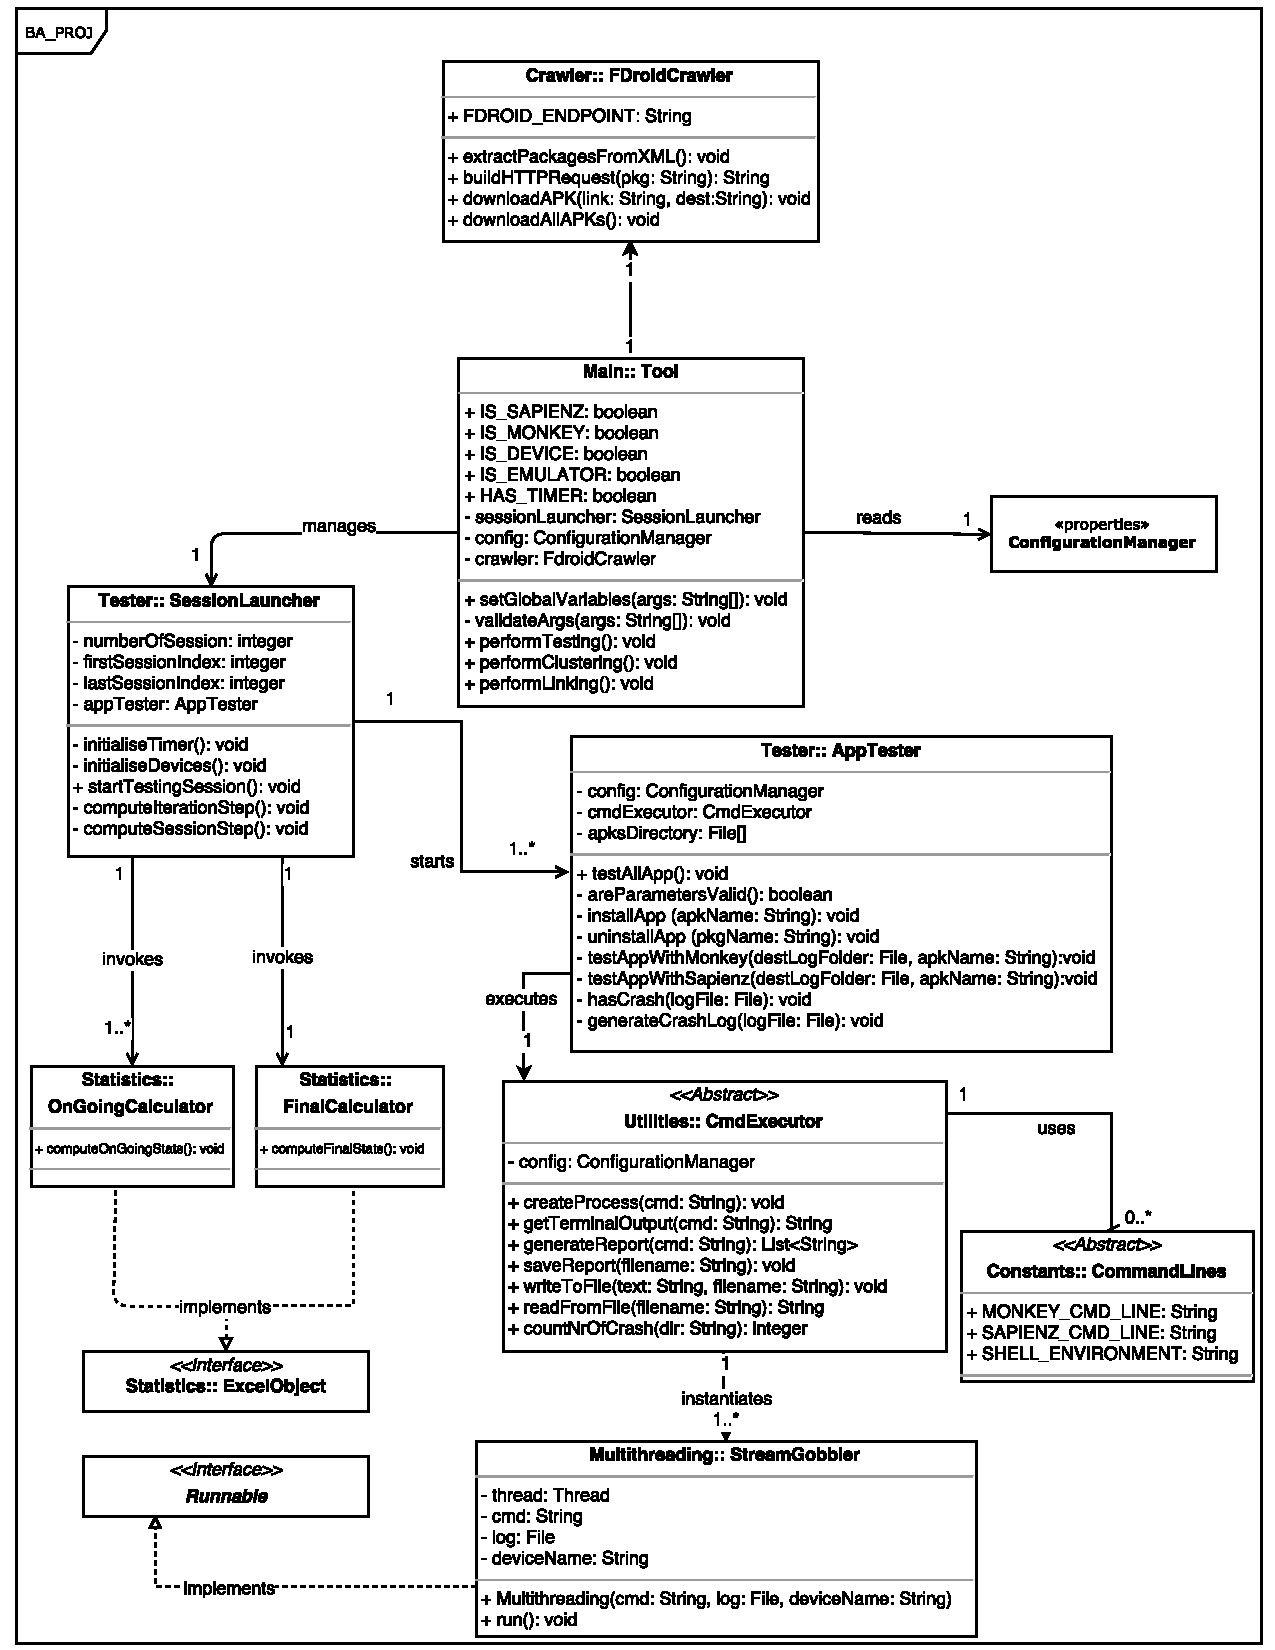
\includegraphics[width=\columnwidth]{diagrams/TesterClassDiagram.pdf} 
\caption{Class Diagram of the testing part of the tool }
\label{testerDiagram}
\vspace{-3mm} 
\end{figure}


Class diagram of the clustering part.
\begin{figure}[t]
\centering 
%	\vspace{-1.5mm} 
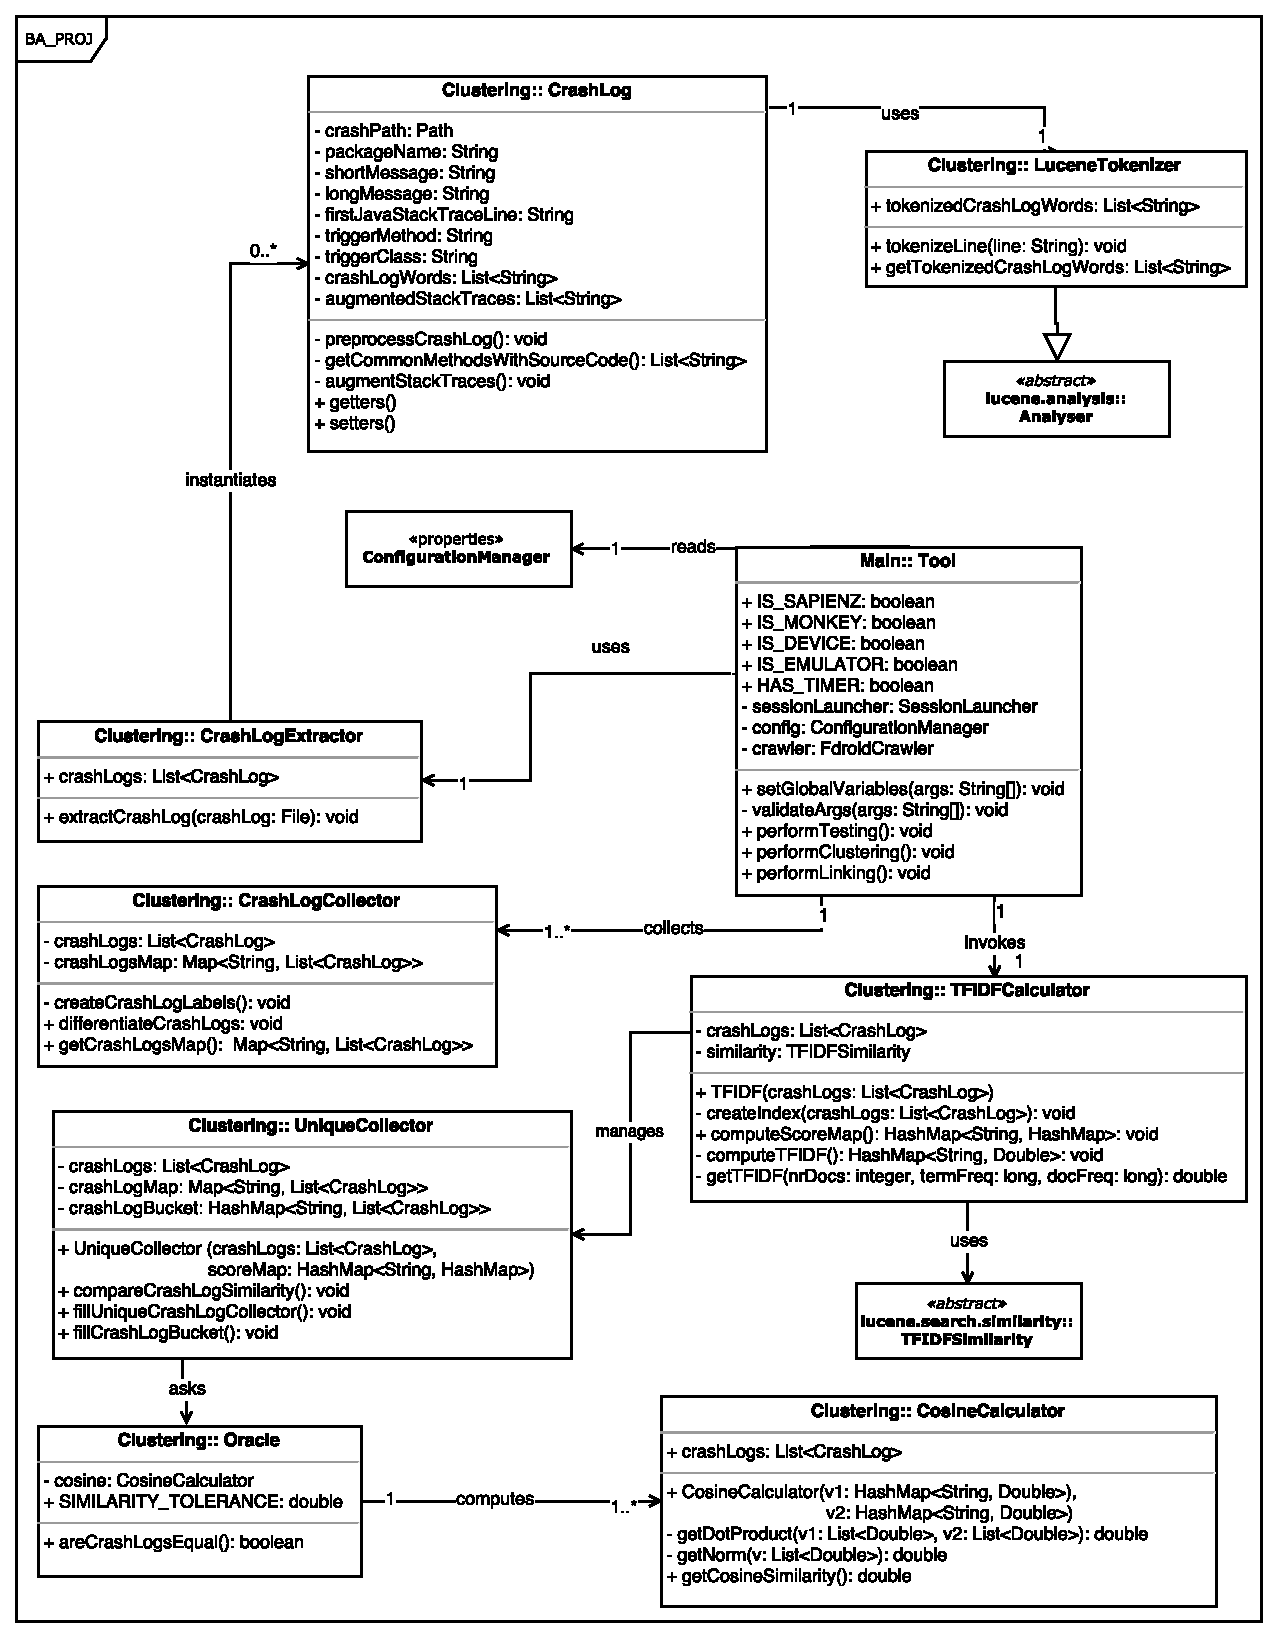
\includegraphics[width=\columnwidth]{diagrams/ClusteringClassDiagram.pdf} 
\caption{Class Diagram of the clustering part of the tool }
\label{cluseringDiagram}
\vspace{-3mm} 
\end{figure}